\documentclass[a4paper,11pt]{article}

% fonts
\usepackage[utf8]{inputenc}
%\usepackage[francais]{babel}

% to get hyphenation on accented words
\usepackage[T1]{fontenc}

% href
\usepackage{hyperref}
\hypersetup{
    colorlinks=true,
    linkcolor=blue,
    filecolor=blue,      
    urlcolor=blue,
    bookmarks=true
}

% code highlighting
\usepackage{minted}
\usemintedstyle{pastie}

% asm
\usepackage{amsmath}
\usepackage{amssymb}
\usepackage{amsthm}

% inline code
\usepackage{listings}
\usepackage{xcolor}

% tables
\usepackage{booktabs}

% algorithm
\usepackage[]{algorithm2e}

% for right cases
\newenvironment{rcases}
  {\left.\begin{aligned}}
  {\end{aligned}\right\rbrace}
  
% images
\usepackage{graphicx}
\usepackage{float}

% diagrams
\usepackage{tikz}
\usetikzlibrary{matrix}
\usetikzlibrary{positioning}

% tables
\usepackage{booktabs}

% no identation
\setlength{\parindent}{0pt}

% theorem
\newtheorem{definition}{Definition}
\newtheorem{property}{Property}
\newtheorem{theorem}{Theorem}

% header
\title{Timing and Lattice Attacks on a Remote ECDSA OpenSSL Server: How Practical Are They Really?}
\author{David Wong}
\date{\emph{University of Bordeaux and NCC Group}, \small{September 2015}}

% 
\begin{document}

\maketitle

\renewcommand{\abstractname}{Abstract}
\begin{abstract}
In 2011, B.B.Brumley and N.Tuveri found a remote timing attack on OpenSSL's ECDSA implementation for binary curves. We will study if the title of their paper was indeed relevant (Remote Timing Attacks are Still Practical). We improved on their lattice attack using the Embedding Strategy that reduces the Closest Vector Problem to the Shortest Vector Problem so as to avoid using Babai's procedures to solve the CVP and rely on the better experimental results of LLL. We will detail (along with publishing the source code of the tools we used) our attempts to reproduce their experiments from a remote machine located on the same network with the server, and see that such attacks are not trivial and far from being practical. Finally we will see other attacks and countermeasures.\\
\\
\textbf{Keywords:} DSA, ECDSA, Timing Attacks, Remote Side-Channel Attacks, OpenSSL, Howgrave-Graham and Smart, B.B.Brumley and N.Tuveri, Hidden Number Problem, Lattices, SVP, CVP, Babai, LLL, BKZ, Embedding Strategy, Short Nonces.\\

\end{abstract}

\section{Introduction}\label{introduction}

Randomness is an intrinsic part of any cryptosystem. It is the source we draw from to generate the secret keys of our Block Ciphers, it is the birthplace of the long keystreams engendered by our Stream Ciphers, the insurance of our Message Authentication Codes and ground zero for our Signatures. Being able to predict the origin of randomness of a cryptosystem will usually break the entirety of it. Using a bad Random Number Generator (\textbf{RNG}) is often the cause of many troubles, this is why nowadays we use the better \textbf{CSPRNGs} (Cryptographically Secure Pseudo Random Number Generators) that enable us to generate random numbers that are not predictable nor reveal any information about the previous random numbers generated (Forward Secrecy). One way of breaking these might be to use a backdoor, like Dual EC\cite{dualec} does, or to leak them through other channels.

In this paper we will show how these ``Side-Channels'' can sometimes provide enough information to break a cryptosystem. In particular, how the knowledge of a few bits of dozens of nonces revealed by a timing attack can break DSA and ECDSA in applications like OpenSSL. In section 2 we will introduce Cryptographic Signatures with brief explanations on DSA and its Elliptic Curve variant ECDSA. In section 3 we will talk a bit about lattices and the interesting problems they carry, along with the tools past research has invented to solve them (or rather approximate them). In section 4 we will see how Howgrave-Graham and Smart attacked DSA with algorithms based on lattices. We will explain in details a special case of their attack: when the nonces are short, and will talk about improvements by using the Embedding Strategy. In section 5 we will start talking about a timing attack found by B.B.Brumley and N.Tuveri that recovers an OpenSSL server's private key by obtaining some information about the length of the nonces of its ECDSA signatures. We will follow by showing how to mount the attack and see how practical it really is according to our own experiments. In section 6 we will talk about related attacks and known counter-measures. Finally we will end the paper with a short conclusion in section 7. In appendix A you will find the C code of the timing part of the attack, in appendix B you will find the Sage code of the lattice part of the attack. Both can be found up to date on \href{https://github.com/mimoo/timing_attack_ecdsa_tls}{the public repository associated to this paper}.

\section{Cryptographic Signatures}\label{rsa}


One of the greatest tool cryptography has provided us in the modern era is the ability to digitally sign things. Like a real signature is ``supposed'' to attest you wrote that check, a digital signature over a digital object can attest it came from you. Actually a digital signature does much more: it \textbf{authenticate} the object (it came from you), it provides \textbf{integrity} (it has not been modified) and also \textbf{non-repudiation} (you cannot lie afterward about not having signed anything!).

\subsection{DSA}\label{dsa}

The Digital Signature Algorithm, commonly referred as DSA or even DSS (the same way Rijandel is referred to as AES), is one of the most used signature algorithms in the world. It is a variant of Schnorr's Signature\cite{schnorr} published by the NSA to circumvent the first one's patents. Based on Non-Interactive Zero-Knowledge Protocols and Public-Key Cryptography, it is pretty simple to state. You own two keys: a public key and a private key. You sign with your private key and people can verify your signature thanks to your public key which is... public.

\begin{align*}
&x \text{ the private key} \\
&(p, q, g, y) \text{ the public key with } y = g^x \pmod{p}
\end{align*}

We will not go into the details of how to generate a pair of private and public key. A signature over a message consists of two integers $r$ and $s$ that you can compute with a hash of the message, your private key, the public key and an \textbf{ephemeral private key} $k$.

\begin{align*}
&r = (g^k \pmod{p}) \pmod{q}\\
&s = k^{-1} ( H(m) + x r ) \pmod{q}
\end{align*}

Every time you want to sign something you must generate a new ephemeral private key $k$ in addition to your long term private key $x$. This is why we also call it a nonce as it is a \textbf{n}umber that has to be used only \textbf{once}.

The verification part is pretty straight forward: take the elements from the signature and from the public key and compute:

$$ (g^{H(m) (s^{-1} \pmod{q})} \cdot g^{r (s^{-1} \pmod{q}) \pmod{q}} \pmod{p}) \pmod{q} $$

Check if it's equal to $r$. If so, the signature is valid.

\subsection{ECDSA}\label{ecdsa}

ECDSA, a more modern variant of DSA based on \textbf{Elliptic Curves}, was invented in 1992 by Scott Vanstone in response to NIST's Request For Comment on their DSA\cite{ecdsa}. It carries better security assumptions and is more efficient than DSA due to smaller key sizes. It has been slowly replacing it over the years.

DSA is based on the \textbf{Discrete Logarithm Problem} (DLP) in prime-order subgroups of $\mathbb{Z}^{\ast}_p$. The fact that given $y = g^x \pmod{p}$ with $g$ an element of the multiplicative group $\mathbb{Z}_{p}^{\ast}$ ($p$ prime), it is \emph{hard} to compute the integer $x$. This problem can be found in other kinds of groups like the one we define with Elliptic Curves, it is then called the \textbf{Elliptic Curve Discrete Logarithm Problem} or ECDLP in some of the fields.\\

Elliptic Curves are just some kind of curves usually defined as the points satisfying the \textbf{Weiestraß' equation} over a field $K$ along with a point $\mathcal{O}$ serving as the identity and called the \textit{point at infinity}:

$$ y^2 + a_1xy + a_3y = x^3 + a_2x^2 + a_4x + a_6 $$

That set of points forms an abelian group along with two operations (addition and multiplication) which are defined following a \textit{chord-and-tangent rule}. The multiplication of a scalar $k$ with a point $P$ from the curve is usually written as $Q = [k]P$. The ECDLP is stated as follow: it is computationally hard to compute $k$ if you only know $Q$ and $P$ in the above equation (and if they are big enough).

The main advantage of ECDLP over DLP is that the most efficients attack on DLP (\textit{Index Calculus} attacks like the \textbf{General Number Field Sieve}) do not work for ECDLP. Keys in Elliptic Curve based algorithms are also much smaller than their counterparts based on conventional the Discrete Logarithm Problem, which allows for faster calculations and smaller certificates for equivalent levels of security. 

ECDSA carries the same principles as DSA. The public key comprises all the public parameters of the curve of our choice and a public key $Q = [x]P$ which is a random multiple $x$ of the base point $P$  where $x$ is also the private key.

\begin{align*}
&r = ([k]P)_x \pmod{q}\\
&s = k^{-1} ( H(m) + x r ) \pmod{q}
\end{align*}

Pay attention to the scalar multiplication in the first part $r$ of the signature. This is the part that we will later talk about.

\subsection{Security of DSA/ECDSA}\label{security_dsa_ecdsa}

The security of DSA and ECDSA are often grossly reduced to the Discrete Logarithm Problem, while it should be tied to every information contained in its equations.

Taking a look at the public part $(r, s)$ of an ECDSA signature:
\begin{align*}
&r = [k] P\\
&s = k^{-1} ( H(m) + x r ) \pmod{q}
\end{align*}

You can see in the second equation that knowing the nonce $k$ allows you to easily recover the private key $x$ (total break):

$$
x = [ s k - H(m) ] \cdot r^{-1} \pmod{q}
$$

An example of a misunderstanding of this concept is the PS3 nonce \textbf{re-use} in 2010\cite{ps3} where a team of researcher reversed the nonce generation part of the PS3 signing algorithm to realize that it was not totally random.

\begin{figure}[H]
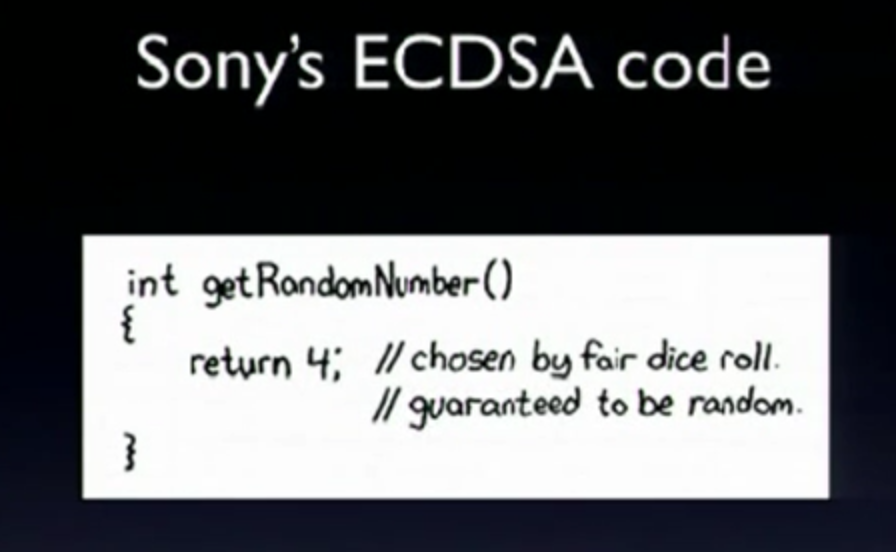
\includegraphics[width=\textwidth]{ps3.png}
\caption{The relevant slide from the \href{https://events.ccc.de/congress/2010/Fahrplan/attachments/1780_27c3_console_hacking_2010.pdf}{Chaos Communication Congress talk revealing the vulnerability}}
\end{figure}

You can see that reusing the same nonce only twice already leads to a break of the key:

\begin{align*}
    &\begin{cases}
    s_1 = k^{-1} ( H(m_1) + x r ) \pmod{q}\\
    s_2 = k^{-1} ( H(m_2) + x r ) \pmod{q}
    \end{cases}\\
\implies& s_1 - s_2 = k^{-1} ( H(m_1) - H(m_2) ) \pmod{q}\\
\implies& k = (H(m_1) - H(m_2)) (s_1 - s_2)^{-1} \pmod{q}
\end{align*}

Nonces being uniformly generated from huge sets make the probability of generating the same nonce twice \textbf{mathematically negligible}. But we will see that we need less information than that. Some subtle information on the nonces, like their \textbf{binary size}, can rapidly lead to the same total break.

\section{Lattices}

The attacks we will describe later both make use of lattices and the tools they carry. Hence it is necessary for us to understand what is a lattice and what algorithms based on lattices will be useful for us.\\
Think about Lattices like \textbf{Vector Spaces}. Imagine a simple vector space of two vectors. You can add them together, multiply them by scalars (let's say numbers of $\mathbb{R}$) and it spans a vector space.\\

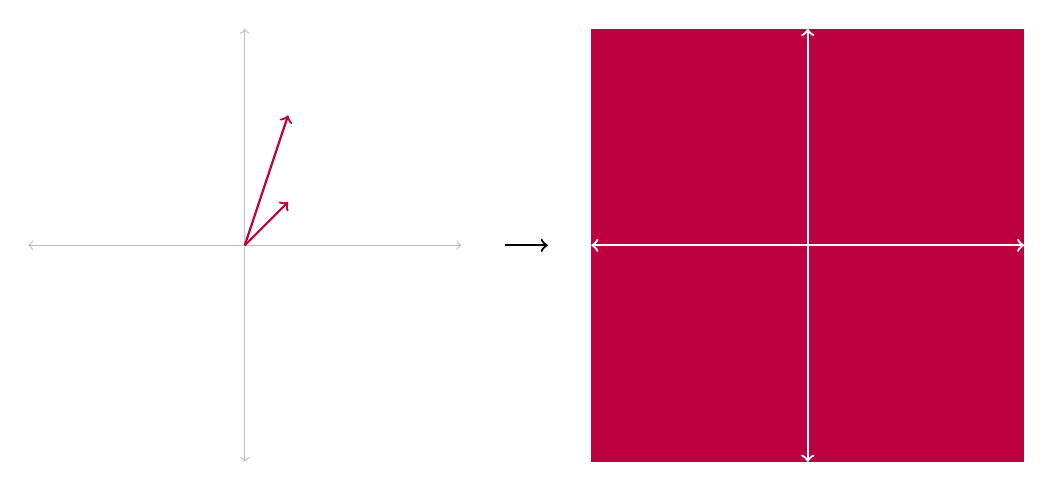
\begin{tikzpicture}[scale=.55]
\draw [lightgray] [<->] (0,5) -- (10,5);
\draw [lightgray] [<->] (5,10) -- (5,0);
\draw [thick,purple] [->] (5,5) -- (6, 8);
\draw [thick,purple] [->] (5,5) -- (6, 6);

\draw [thick,black] [->] (11,5) -- (12,5);

%\path [fill=purple] (18,5) to (20.5,10) to (23,10) to (18,5);
\path [fill=purple] (13,0) to (23,0) to (23,10) to (13,10);
\draw [white,thick] [<->] (13,5) -- (23,5);
\draw [white,thick] [<->] (18,10) -- (18,0);
\end{tikzpicture}\\

Now imagine that our vector space's \textbf{scalars are the integers}, taken in $\mathbb{Z}$. The space spanned by the vectors is now made out of points. It's \textbf{discrete}. Meaning that for any point of this lattice there exists a ball centered around that point of radius different from zero that contains only that point. Nothing else.\\

\begin{figure}[H]
\centering
\begin{tikzpicture}[scale=.5]
\draw [lightgray] [<->] (0,5) -- (10,5);
\draw [lightgray] [<->] (5,10) -- (5,0);

\draw [fill,purple] (9,1) circle [radius=0.1];

\draw [fill,purple] (7,1) circle [radius=0.1];
\draw [fill,purple] (8,2) circle [radius=0.1];
\draw [fill,purple] (9,3) circle [radius=0.1];

\draw [fill,purple] (5,1) circle [radius=0.1];
\draw [fill,purple] (6,2) circle [radius=0.1];
\draw [fill,purple] (7,3) circle [radius=0.1];
\draw [fill,purple] (8,4) circle [radius=0.1];
\draw [fill,purple] (9,5) circle [radius=0.1];

\draw [fill,purple] (3,1) circle [radius=0.1];
\draw [fill,purple] (4,2) circle [radius=0.1];
\draw [fill,purple] (5,3) circle [radius=0.1];
\draw [fill,purple] (6,4) circle [radius=0.1];
\draw [fill,purple] (7,5) circle [radius=0.1];
\draw [fill,purple] (8,6) circle [radius=0.1];
\draw [fill,purple] (9,7) circle [radius=0.1];

\draw [fill,purple] (1,1) circle [radius=0.1];
\draw [fill,purple] (2,2) circle [radius=0.1];
\draw [fill,purple] (3,3) circle [radius=0.1];
\draw [fill,purple] (4,4) circle [radius=0.1];
\draw [fill,purple] (5,5) circle [radius=0.1];
\draw [fill,purple] (6,6) circle [radius=0.1];
\draw [fill,purple] (7,7) circle [radius=0.1];
\draw [fill,purple] (8,8) circle [radius=0.1];
\draw [fill,purple] (9,9) circle [radius=0.1];

\draw [fill,purple] (1,3) circle [radius=0.1];
\draw [fill,purple] (2,4) circle [radius=0.1];
\draw [fill,purple] (3,5) circle [radius=0.1];
\draw [fill,purple] (4,6) circle [radius=0.1];
\draw [fill,purple] (5,7) circle [radius=0.1];
\draw [fill,purple] (6,8) circle [radius=0.1];
\draw [fill,purple] (7,9) circle [radius=0.1];

\draw [fill,purple] (1,5) circle [radius=0.1];
\draw [fill,purple] (2,6) circle [radius=0.1];
\draw [fill,purple] (3,7) circle [radius=0.1];
\draw [fill,purple] (4,8) circle [radius=0.1];
\draw [fill,purple] (5,9) circle [radius=0.1];

\draw [fill,purple] (1,7) circle [radius=0.1];
\draw [fill,purple] (2,8) circle [radius=0.1];
\draw [fill,purple] (3,9) circle [radius=0.1];

\draw [fill,purple] (1,9) circle [radius=0.1];
\end{tikzpicture}
\end{figure}

Lattice are interesting in cryptography because we seldom deal with real numbers and they bring us a lot of tools to deal with integers.

Just as vector spaces, lattices can also be described by different basis represented as \textbf{matrices}. 

Lattices come with their sets of hard problems, and in our interest their respective approximation-to-a-solution tools.

\subsection{Shortest Vector Problem}

One of the most famous lattice problems thought to be hard is the \textbf{SVP} or Shortest Vector Problem. It states that given a lattice basis, you have to find the shortest non-zero vector in the lattice.

\begin{figure}[H]
  \centering
  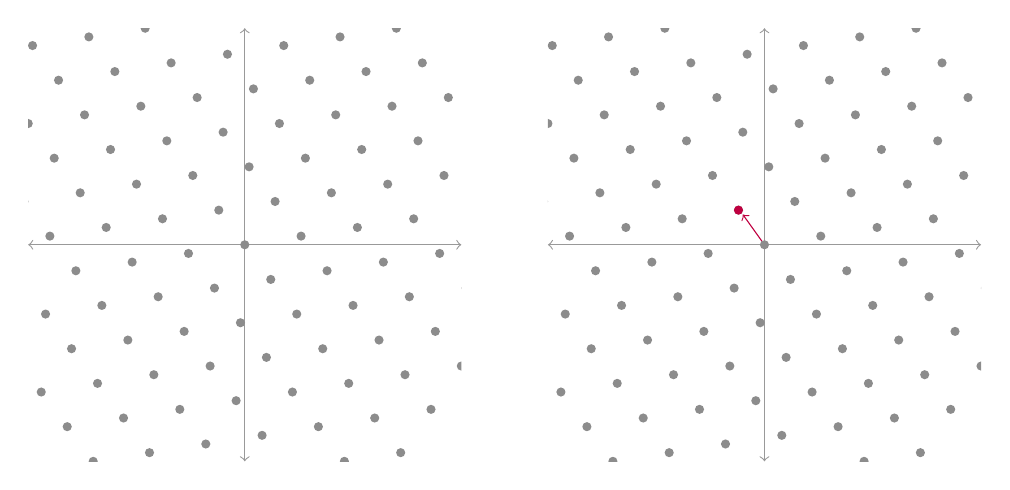
\begin{tikzpicture}[scale=1]
  
  
  \begin{scope}[scale=.55,local bounding box=scope1]
        \coordinate (Origin)   at (0,0);
        \coordinate (XAxisMin) at (-5,0);
        \coordinate (XAxisMax) at (5,0);
        \coordinate (YAxisMin) at (0,-5);
        \coordinate (YAxisMax) at (0,5);
        \draw [thin, black!40, <->] (XAxisMin) -- (XAxisMax);% Draw x axis
        \draw [thin, black!40,<->] (YAxisMin) -- (YAxisMax);% Draw y axis
        %\draw[style=help lines,dashed,black!20] (-5,-5) grid[step=1cm] (5,5);
        
      
        \begin{scope}
            \clip (-5,-5) rectangle (5,5); % Clips the picture...
            \pgftransformcm{1}{0.6}{0.7}{1}{\pgfpoint{0cm}{0cm}}
        
            % setup the nodes
            \foreach \x in {-15,...,15}
            \foreach \y in {-15,...,15}
            {
                \node[shape=circle,fill=black!45,scale=0.35] (\x-\y) at (2*\x,\y+3){};
            }
        \end{scope}
        
    
    \end{scope}
    
  \begin{scope}[scale=.55,shift={(12,0)}]
        \coordinate (Origin)   at (0,0);
        \coordinate (XAxisMin) at (-5,0);
        \coordinate (XAxisMax) at (5,0);
        \coordinate (YAxisMin) at (0,-5);
        \coordinate (YAxisMax) at (0,5);
        \draw [thin, black!40, <->] (XAxisMin) -- (XAxisMax);% Draw x axis
        \draw [thin, black!40,<->] (YAxisMin) -- (YAxisMax);% Draw y axis
        \draw [thin, purple,->] (0,0) -- (-.5,.7);
        %\draw[style=help lines,dashed,black!20] (-5,-5) grid[step=1cm] (5,5);
        
      
        \begin{scope}
            \clip (-5,-5) rectangle (5,5); % Clips the picture...
            \pgftransformcm{1}{0.6}{0.7}{1}{\pgfpoint{0cm}{0cm}}
        
            % setup the nodes
            \foreach \x in {-15,...,15}
            \foreach \y in {-15,...,15}
            {
                \node[shape=circle,fill=black!45,scale=0.35] (\x-\y) at (2*\x,\y+3){};
            }
        \end{scope}
        
        % our little node
        \node[shape=circle,fill=purple,scale=0.35] at (-.6,.8){};
    
    \end{scope}

  \end{tikzpicture}
  \caption{To solve the SVP problem find the shortest lattice vector in that lattice}
\end{figure}

This problem might seem obvious in the example, but lattice basis are rarely optimal and in more dimensions and/or with a bigger basis it quickly becomes problematic to solve the SVP.

\subsection{Closest Vector Problem}

Another interesting problem in lattices is the \textbf{CVP} or Closest Vector Problem, where given a lattice basis and a non-lattice vector you have to find the closest lattice vector to it.

\begin{figure}[H]
  \centering
  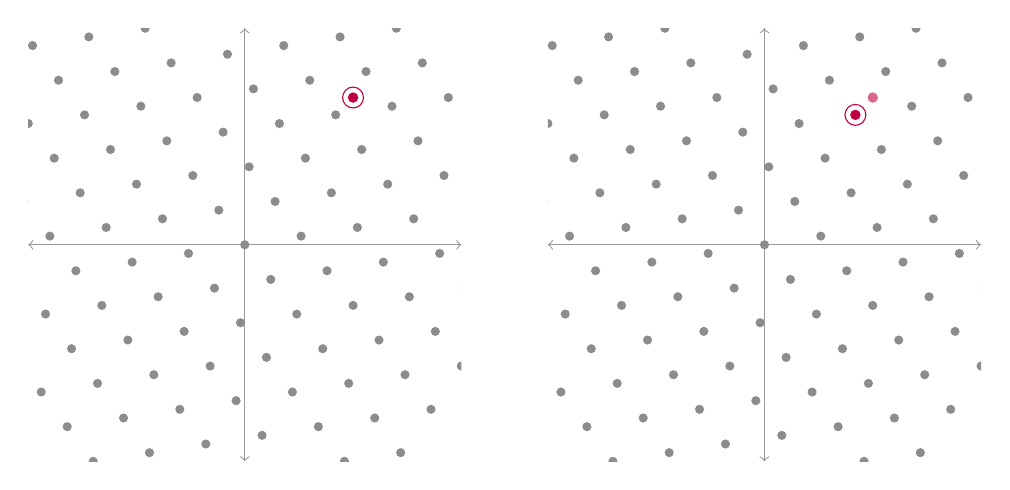
\begin{tikzpicture}[scale=1]
  
  
  \begin{scope}[scale=.55,local bounding box=scope1]
        \coordinate (Origin)   at (0,0);
        \coordinate (XAxisMin) at (-5,0);
        \coordinate (XAxisMax) at (5,0);
        \coordinate (YAxisMin) at (0,-5);
        \coordinate (YAxisMax) at (0,5);
        \draw [thin, black!40, <->] (XAxisMin) -- (XAxisMax);% Draw x axis
        \draw [thin, black!40,<->] (YAxisMin) -- (YAxisMax);% Draw y axis
        %\draw[style=help lines,dashed,black!20] (-5,-5) grid[step=1cm] (5,5);
        
      
        \begin{scope}
            \clip (-5,-5) rectangle (5,5); % Clips the picture...
            \pgftransformcm{1}{0.6}{0.7}{1}{\pgfpoint{0cm}{0cm}}
        
            % setup the nodes
            \foreach \x in {-15,...,15}
            \foreach \y in {-15,...,15}
            {
                \node[shape=circle,fill=black!45,scale=0.35] (\x-\y) at (2*\x,\y+3){};
            }
        \end{scope}
        
        % our little node
        \node[shape=circle,fill=purple,scale=0.4] at (2.5,3.4){};
        \node[shape=circle,draw=purple,fill=none,scale=0.8] at (2.5,3.4){};
        
    
    \end{scope}
    
  \begin{scope}[scale=.55,shift={(12,0)}]
        \coordinate (Origin)   at (0,0);
        \coordinate (XAxisMin) at (-5,0);
        \coordinate (XAxisMax) at (5,0);
        \coordinate (YAxisMin) at (0,-5);
        \coordinate (YAxisMax) at (0,5);
        \draw [thin, black!40, <->] (XAxisMin) -- (XAxisMax);% Draw x axis
        \draw [thin, black!40,<->] (YAxisMin) -- (YAxisMax);% Draw y axis
        %\draw[style=help lines,dashed,black!20] (-5,-5) grid[step=1cm] (5,5);
        
      
        \begin{scope}
            \clip (-5,-5) rectangle (5,5); % Clips the picture...
            \pgftransformcm{1}{0.6}{0.7}{1}{\pgfpoint{0cm}{0cm}}
        
            % setup the nodes
            \foreach \x in {-15,...,15}
            \foreach \y in {-15,...,15}
            {
                \node[shape=circle,fill=black!45,scale=0.35] (\x-\y) at (2*\x,\y+3){};
            }
        \end{scope}
        
        % our little node
        \node[shape=circle,fill=purple!60,scale=0.4] at (2.5,3.4){};
        \node[shape=circle,fill=purple,scale=0.4] at (2.1,3){};
        \node[shape=circle,fill=none,draw=purple,scale=0.8] at (2.1,3){};
    
    \end{scope}

  \end{tikzpicture}
  \caption{To solve the CVP problem you need to find the closest lattice vector to that non-lattice purple vector}
\end{figure}

Interestingly, The CVP is a generalization of the SVP. The reduction is pretty easy, although not obvious since asking for the closest lattice vector to $0$ would be $0$. This will be left as an exercise for the reader.

\subsection{LLL}


The \textbf{Lenstra–Lenstra–Lovász} \textit{lattice basis reduction algorithm} is a step by step calculus that reduces a lattice basis in polynomial time. The lattice is left unchanged but the row vectors of its new basis are ``\textbf{smaller}'' and nearly orthogonal to one another. Here's the real definitions:

\begin{definition}
Let $L$ be a lattice with a basis $B$. The $\delta$-LLL algorithm applied on $L$'s basis $B$ produces a new basis of $L$: $B' = \{b_1,\hdots,b_n\}$ satisfying:
\begin{eqnarray}
\forall \hspace{1mm} 1 \leq j < i \leq n \text{ we have } |\mu_{i,j}| \leq \frac{_1}{^2}\\
\forall \hspace{1mm} 1 \leq i < n \text{ we have } \delta \cdot \|\tilde{b_i}\|^2 \leq \| \mu_{i+1,i}\cdot \tilde{b}_i + \tilde{b}_{i + 1}\|^2
\end{eqnarray}
\begin{center}
with $\mu_{i,j} = \frac{b_i \cdot \tilde{b}_j}{\tilde{b}_j \cdot \tilde{b}_j}$ and $\tilde{b}_1 = b_1$ (Gram-Schmidt)
\end{center}
\end{definition}

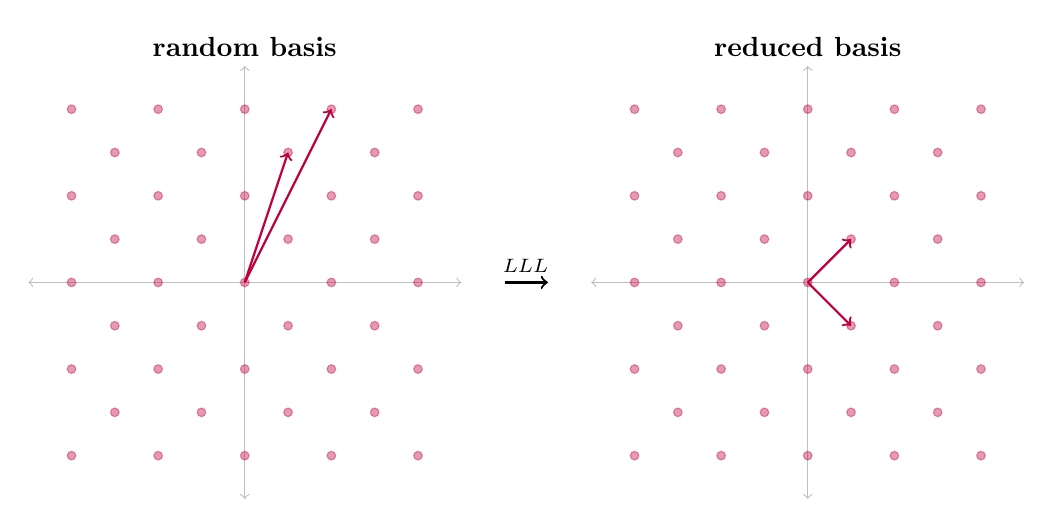
\begin{tikzpicture}[scale=.55]
\node [above] at (5,10) {\textbf{random basis}};
\node [above] at (18,10) {\textbf{reduced basis}};
\draw [lightgray] [<->] (0,5) -- (10,5);
\draw [lightgray] [<->] (5,10) -- (5,0);

\draw [fill,purple,opacity=.4] (9,1) circle [radius=0.1];

\draw [fill,purple,opacity=.4] (7,1) circle [radius=0.1];
\draw [fill,purple,opacity=.4] (8,2) circle [radius=0.1];
\draw [fill,purple,opacity=.4] (9,3) circle [radius=0.1];

\draw [fill,purple,opacity=.4] (5,1) circle [radius=0.1];
\draw [fill,purple,opacity=.4] (6,2) circle [radius=0.1];
\draw [fill,purple,opacity=.4] (7,3) circle [radius=0.1];
\draw [fill,purple,opacity=.4] (8,4) circle [radius=0.1];
\draw [fill,purple,opacity=.4] (9,5) circle [radius=0.1];

\draw [fill,purple,opacity=.4] (3,1) circle [radius=0.1];
\draw [fill,purple,opacity=.4] (4,2) circle [radius=0.1];
\draw [fill,purple,opacity=.4] (5,3) circle [radius=0.1];
\draw [fill,purple,opacity=.4] (6,4) circle [radius=0.1];
\draw [fill,purple,opacity=.4] (7,5) circle [radius=0.1];
\draw [fill,purple,opacity=.4] (8,6) circle [radius=0.1];
\draw [fill,purple,opacity=.4] (9,7) circle [radius=0.1];

\draw [fill,purple,opacity=.4] (1,1) circle [radius=0.1];
\draw [fill,purple,opacity=.4] (2,2) circle [radius=0.1];
\draw [fill,purple,opacity=.4] (3,3) circle [radius=0.1];
\draw [fill,purple,opacity=.4] (4,4) circle [radius=0.1];
\draw [fill,purple,opacity=.4] (5,5) circle [radius=0.1];
\draw [fill,purple,opacity=.4] (6,6) circle [radius=0.1];
\draw [fill,purple,opacity=.4] (7,7) circle [radius=0.1];
\draw [fill,purple,opacity=.4] (8,8) circle [radius=0.1];
\draw [fill,purple,opacity=.4] (9,9) circle [radius=0.1];

\draw [fill,purple,opacity=.4] (1,3) circle [radius=0.1];
\draw [fill,purple,opacity=.4] (2,4) circle [radius=0.1];
\draw [fill,purple,opacity=.4] (3,5) circle [radius=0.1];
\draw [fill,purple,opacity=.4] (4,6) circle [radius=0.1];
\draw [fill,purple,opacity=.4] (5,7) circle [radius=0.1];
\draw [fill,purple,opacity=.4] (6,8) circle [radius=0.1];
\draw [fill,purple,opacity=.4] (7,9) circle [radius=0.1];

\draw [fill,purple,opacity=.4] (1,5) circle [radius=0.1];
\draw [fill,purple,opacity=.4] (2,6) circle [radius=0.1];
\draw [fill,purple,opacity=.4] (3,7) circle [radius=0.1];
\draw [fill,purple,opacity=.4] (4,8) circle [radius=0.1];
\draw [fill,purple,opacity=.4] (5,9) circle [radius=0.1];

\draw [fill,purple,opacity=.4] (1,7) circle [radius=0.1];
\draw [fill,purple,opacity=.4] (2,8) circle [radius=0.1];
\draw [fill,purple,opacity=.4] (3,9) circle [radius=0.1];

\draw [fill,purple,opacity=.4] (1,9) circle [radius=0.1];

%
\draw [thick,black] [->] (11,5) -- (12,5);
\node [above] at (11.5,5) {$_{LLL}$};
%

\draw [lightgray] [<->] (13,5) -- (23,5);
\draw [lightgray] [<->] (18,10) -- (18,0);

\draw [fill,purple,opacity=.4] (22,1) circle [radius=0.1];

\draw [fill,purple,opacity=.4] (20,1) circle [radius=0.1];
\draw [fill,purple,opacity=.4] (21,2) circle [radius=0.1];
\draw [fill,purple,opacity=.4] (22,3) circle [radius=0.1];

\draw [fill,purple,opacity=.4] (18,1) circle [radius=0.1];
\draw [fill,purple,opacity=.4] (19,2) circle [radius=0.1];
\draw [fill,purple,opacity=.4] (20,3) circle [radius=0.1];
\draw [fill,purple,opacity=.4] (21,4) circle [radius=0.1];
\draw [fill,purple,opacity=.4] (22,5) circle [radius=0.1];

\draw [fill,purple,opacity=.4] (16,1) circle [radius=0.1];
\draw [fill,purple,opacity=.4] (17,2) circle [radius=0.1];
\draw [fill,purple,opacity=.4] (18,3) circle [radius=0.1];
\draw [fill,purple,opacity=.4] (19,4) circle [radius=0.1];
\draw [fill,purple,opacity=.4] (20,5) circle [radius=0.1];
\draw [fill,purple,opacity=.4] (21,6) circle [radius=0.1];
\draw [fill,purple,opacity=.4] (22,7) circle [radius=0.1];

\draw [fill,purple,opacity=.4] (14,1) circle [radius=0.1];
\draw [fill,purple,opacity=.4] (15,2) circle [radius=0.1];
\draw [fill,purple,opacity=.4] (16,3) circle [radius=0.1];
\draw [fill,purple,opacity=.4] (17,4) circle [radius=0.1];
\draw [fill,purple,opacity=.4] (18,5) circle [radius=0.1];
\draw [fill,purple,opacity=.4] (19,6) circle [radius=0.1];
\draw [fill,purple,opacity=.4] (20,7) circle [radius=0.1];
\draw [fill,purple,opacity=.4] (21,8) circle [radius=0.1];
\draw [fill,purple,opacity=.4] (22,9) circle [radius=0.1];

\draw [fill,purple,opacity=.4] (14,3) circle [radius=0.1];
\draw [fill,purple,opacity=.4] (15,4) circle [radius=0.1];
\draw [fill,purple,opacity=.4] (16,5) circle [radius=0.1];
\draw [fill,purple,opacity=.4] (17,6) circle [radius=0.1];
\draw [fill,purple,opacity=.4] (18,7) circle [radius=0.1];
\draw [fill,purple,opacity=.4] (19,8) circle [radius=0.1];
\draw [fill,purple,opacity=.4] (20,9) circle [radius=0.1];

\draw [fill,purple,opacity=.4] (14,5) circle [radius=0.1];
\draw [fill,purple,opacity=.4] (15,6) circle [radius=0.1];
\draw [fill,purple,opacity=.4] (16,7) circle [radius=0.1];
\draw [fill,purple,opacity=.4] (17,8) circle [radius=0.1];
\draw [fill,purple,opacity=.4] (18,9) circle [radius=0.1];

\draw [fill,purple,opacity=.4] (14,7) circle [radius=0.1];
\draw [fill,purple,opacity=.4] (15,8) circle [radius=0.1];
\draw [fill,purple,opacity=.4] (16,9) circle [radius=0.1];

\draw [fill,purple,opacity=.4] (14,9) circle [radius=0.1];

% vectors
\draw [thick,purple] [->] (5,5) -- (7, 9);
\draw [thick,purple] [->] (5,5) -- (6, 8);

\draw [thick,purple] [->] (18,5) -- (19, 4);
\draw [thick,purple] [->] (18,5) -- (19, 6);
\end{tikzpicture}\\

We will not dig into the internals of LLL here, see Chris Peikert's course\cite{chrispeikert} for detailed explanations of the algorithm.

\subsection{Babai}

In 1986, Babai introduced two algorithms\cite{babai} to get an approximation of the Closest Vector Problem.\\
Let $L$ be a lattice in $\mathbb{R}^d$, given by a basis $B = {b_1, \hdots, b_d}$ and let $x \in \mathbb{R}^d$. Let $u$ be the nearest neighbor of $x$ in $L$. Babai's procedures bring a way to find an approximation $w$ of this vector $u$.

\textbf{Rounding Off procedure:} Let $x = \sum^d_{i=1} \beta_i b_i$ and let $\alpha_i$ be the integer nearest to $\beta_i$. Set $w = \sum^d_{i=1} \alpha_i b_i$.\\

\textbf{Nearest Plane procedure:} Let $U = \sum^{d-1}_{i=1} R b_i$ be the linear subspace generated by $b_1, \hdots, b_{d-1}$ and let $L' = \sum^{d-1}_{i=1} Z b_i$ be the corresponding sublattice of $L$.\\
Find $v \in L$ such that the distance between $x$ and the affine subspace $U + v$ be minimal. Let $x'$ denote the orthogonal projection of $x$ on $U + v$. Recursively, find $y \in L'$ near $x' - v$. Let $w = y + v$.\\
In order to find $v$ and $x'$, we proceed as follows:
\begin{itemize}
\item Write $x$ as a linear combination of the orthogonal basis: $x = \sum^{d}_{i=1} \gamma_i b_i^{\ast}$.
\item Let $\delta$ be the integer nearest to $\gamma_d$.
\item Then $x' = \sum^{d-1}_{i=1} \gamma b_i^{\ast} + \delta b_d^{\ast}$ and $v = \delta b_d$.
\end{itemize}

The \textbf{Rounding Off procedure} is simple enough to be explained here:

\begin{figure}[H]
  \centering
  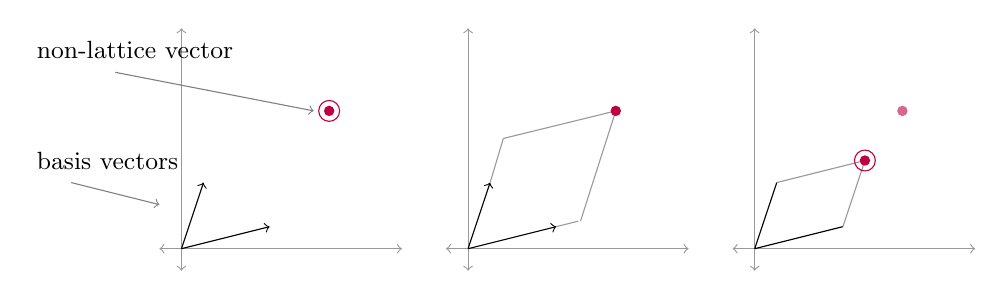
\begin{tikzpicture}[scale=1]
  
  
  \begin{scope}[scale=.28,local bounding box=scope1]
        \coordinate (Origin)   at (0,0);
        \coordinate (XAxisMin) at (-1,0);
        \coordinate (XAxisMax) at (10,0);
        \coordinate (YAxisMin) at (0,-1);
        \coordinate (YAxisMax) at (0,10);
        \draw [thin, black!40, <->] (XAxisMin) -- (XAxisMax);% Draw x axis
        \draw [thin, black!40,<->] (YAxisMin) -- (YAxisMax);% Draw y axis
        %\draw[style=help lines,dashed,black!20] (-5,-5) grid[step=1cm] (5,5);
        
        % basis vectors
        \draw [->] (Origin) -- (4,1);
        \draw [->] (Origin) -- (1,3);
        
        % explanation
        \node[right] at (-7, 9) {\small{non-lattice vector}};
        \draw[->, black!50] (-3, 8) -- (6,6.25);
        
        \node[right] at (-7, 4) {\small{basis vectors}};
        \draw[->, black!50] (-5, 3) -- (-1, 2);
        
        % our little node
        \node[shape=circle,fill=purple,scale=0.4] at (6.7,6.25){};
        \node[shape=circle,draw=purple,fill=none,scale=0.8] at (6.7,6.25){};
        
    
    \end{scope}
    
  \begin{scope}[scale=.28,shift={(13,0)}]
        \coordinate (Origin)   at (0,0);
        \coordinate (XAxisMin) at (-1,0);
        \coordinate (XAxisMax) at (10,0);
        \coordinate (YAxisMin) at (0,-1);
        \coordinate (YAxisMax) at (0,10);
        \draw [thin, black!40, <->] (XAxisMin) -- (XAxisMax);% Draw x axis
        \draw [thin, black!40,<->] (YAxisMin) -- (YAxisMax);% Draw y axis
        %\draw[style=help lines,dashed,black!20] (-5,-5) grid[step=1cm] (5,5);
        
        % basis vectors
        \draw [->] (Origin) -- (4,1);
        \draw [->] (Origin) -- (1,3);
        
        % extended basis vectors
        \draw [black!40] (4,1) -- (5,1.25);
        \draw [black!40] (1,3) -- (1.6,5);
        
        \draw [black!40] (5.1,1.25) -- (6.7,6.25);
        \draw [black!40] (1.6,5) -- (6.7,6.25);
        
        %\draw [black!40] (4,1) -- (5,4);
        %\draw [black!40] (1,3) -- (5,4);
        
        % our little node
        \node[shape=circle,fill=purple,scale=0.4] at (6.7,6.25){};
    
    \end{scope}
    
    
  \begin{scope}[scale=.28,shift={(26,0)}]
        \coordinate (Origin)   at (0,0);
        \coordinate (XAxisMin) at (-1,0);
        \coordinate (XAxisMax) at (10,0);
        \coordinate (YAxisMin) at (0,-1);
        \coordinate (YAxisMax) at (0,10);
        \draw [thin, black!40, <->] (XAxisMin) -- (XAxisMax);% Draw x axis
        \draw [thin, black!40,<->] (YAxisMin) -- (YAxisMax);% Draw y axis
        %\draw[style=help lines,dashed,black!20] (-5,-5) grid[step=1cm] (5,5);
        
        % basis vectors
        \draw (Origin) -- (4,1);
        \draw (Origin) -- (1,3);
        
        % extended basis vectors
        \draw [black!40] (4,1) -- (5,4);
        \draw [black!40] (1,3) -- (5,4);
        
        % our little node
        \node[shape=circle,fill=purple!60,scale=0.4] at (6.7,6.25){};
        
        % our new little node :)
        \node[shape=circle,fill=purple,scale=0.4] at (5,4){};
        \node[shape=circle,fill=none,draw=purple,scale=0.8] at (5,4){};
    
    \end{scope}

  \end{tikzpicture}
  \caption{The non-lattice vector can be written with the basis vectors of the lattice, then the procedure rounds off these coefficients to find the closest lattice vector}
\end{figure}

\section{Lattice Attacks on DSA}

Lattices and the tools they come with have been used everywhere in crypto: building security proofs, building cryptosystems (and sometimes post quantum cryptosystems), breaking cryptosystems.

In 1982, the first efficient lattice basis reduction algorithm LLL was invented by the Lenstra brothers and Lovász\cite{lll}. More than 10 years later, in 1995, Coppersmith was publishing his theorem along with a construction using LLL that could be used to attack RSA\cite{coppersmith}.

A year later, In 1996, D. Boneh and R. Venkatesan\cite{boneh-venkatesan} formulated the \textbf{Hidden Number Problem} and used that same algorithm to construct a proof on Diffie-Hellman and other related algorithms, which is thought by many cryptographers as one of the most positive applications of lattices.

The same kind of idea was independently found by \textbf{Howgrave-Graham} and \textbf{Smart} three years later\cite{HG-smart}, but this time used to attack DSA. Oddly, they made use of Babai's algorithm while a more efficient technique called the Embedding Strategy was used in the paper by Boneh and Venkatesan.

Following is an explanation of a special case of Howgrave-Graham and Smart's attack on DSA, that we will later use to attack ECDSA. We will then explain how to improve on it by using the Embedding Technique.

\subsection{Reducing a Relaxed DSA Problem to a Closest Vector Problem}

So now imagine that \textbf{we have a number $n$ of signatures} $(r,s)$ from DSA that \textbf{all have particularly ``small'' nonces} $k_i$.\\
Recall these are the equations we now have, for $i \in \mathbb{Z}_n$:
\begin{align*}
&r_i = (g^k_i \pmod{p}) \pmod{q}\\
&s_i = k_i^{-1} ( H(m_i) + x \cdot r_i ) \pmod{q}
\end{align*}

Where $g$, $p$, $q$ are public and $H(m_i)$ can be computed as well. Here, the $k_i$ are the secret nonces, $x$ is the private key.

We notice that we know another way of writing \textbf{the second equation} since we know $H(m_i)$:

$$ H(m_i) = s_i k_i - x \cdot r_i \pmod{q} $$

As this is an attack on the nonces we want to \textbf{get rid of the private key}. To do that we will notice that we can use one of the equations and remove it from the others, let's say we can use the first equation:

\begin{align*}
&H(m_0) = s_0 \cdot k_0 - x \cdot r_0 \pmod{q}\\
\forall i, \text{ } &H(m_0) \cdot r_0^{-1} \cdot r_i = s_0 \cdot k_0 \cdot r_0^{-1} \cdot r_i - x \cdot r_i \pmod{q}
\end{align*}

Since we know all the $r_i$ we can compute the second equation, and we can then use it to remove the private key $x$ from all the other equations:

\begin{align*}
\forall i \neq 0 \text{, } H(m_i) - H(m_0) \cdot r_0^{-1} \cdot r_i &= s_i \cdot k_i - s_0 \cdot k_0 \cdot r_0^{-1} \cdot r_i \pmod{q}\\
(H(m_i) - H(m_0) \cdot r_0^{-1} \cdot r_i) \cdot s_i^{-1} &= k_i - k_0 \cdot s_0 \cdot r_0^{-1} \cdot r_i \cdot s_i^{-1} \pmod{q}
\end{align*}

We know have $n - 1$ equations with \textbf{only two unknowns}: the nonces $k_i$ and the nonce of the first equation $k_0$, which should all be around the same size which is relatively \textbf{small}.

$$ k_i + A_i k_0 + B_i = 0 \pmod{q} $$

We have now successfully \textbf{avoided to attack the discrete logarithm} part of the system and reduced it to finding small solutions to a set of modular equations. This is where lattices are useful. We know have to shape our equations to reduce our problem to a CVP or SVP and use any of the algorithm previously talked about.

We now have a system with $k_i < q \text{ } \forall i \in \mathbb{Z}_n$
$$ \begin{cases}
k_0\\
k_1 = - A_1 k_0 + z_1 q - B_1 \\
\hdots\\
k_{n-1} = - A_{n-1} k_0 + z_{n-1} q - B_{n-1}\\
\end{cases}
$$

And if the $k_i$ are small we know that the distance between the $-A_i k_0 + z_i q$ and $Bi$ are small. How can we transform that in a lattice problem? More accurately in a Closest Vector Problem? First let's \textbf{transform the above system into a matrix system}:

$$
\begin{pmatrix} k_0\\k_1\\ \vdots\\k_{n-1} \end{pmatrix} 
=
\begin{pmatrix}
-1\\
A_1 & q  \\
\vdots & & \ddots \\
A_{n-1} & & & q
\end{pmatrix}
\begin{pmatrix} -k_0\\z_1\\ \vdots\\z_{n-1} \end{pmatrix}
- 
\begin{pmatrix} 0\\B_1\\ \vdots\\B_{n-1} \end{pmatrix}
$$

It is now clear that we can use the $n \times n$ matrix as a lattice in which we are looking for a vector (which is the integer linear combinations done with the coefficient vector $(-k_0, z_1, \hdots, z_{n-1})$) that should be very close to the vector $(0, B_1 , \hdots, B_{n-1})$ since their distance is the small vector $(k_0, \hdots, k_{n-1})$.

In other words, we need to find a vector from the lattice spanned by the columns of the above $n \times n$ matrix that is closed to our non-lattice vector $(0, B_1 , \hdots, B_{n-1})$. This will allow us to compute the coefficient vector $(-k_0, z_1, \hdots, z_{n-1})$ which then would allow us to compute the nonces vector $(k_0, \hdots, k_{n-1})$. \textbf{This is an instance of the Closest Vector Problem}, we can then use one of Babai's procedure to try to solve it. Since these algorithms only promise approximations, these ways of finding the nonces are heuristics and not proven. Different lattices will give different outcomes, but as it is known, LLL often yields better results than expected.

\subsection{The Embedding Strategy}

While Howgrave-Graham and Smart talk about using the Babai procedure to solve the CVP, our tests show that it is not efficient enough. The well-known ``Embedding Strategy'' allows to heuristically reduce the CVP problem to the SVP problem and thus directly make use of a lattice basis reduction algorithm to solve the problem (like LLL).

This is how it works: we add our non-lattice vector $u$ in the basis, so that it is now part of the lattice. Remember, we are looking for a very close lattice vector $v$ to our non-lattice vector $u$, since both these vectors are in the lattice, we hope that our reduction algorithm will find $u - v$ or $v - u$ which is in our lattice and should be really small, the heuristic also says to increase the lattice's dimension and to only give a coefficient of the new dimension to our new basis vector $u$. This way we can test if our solution has used our vector $u$ by checking if the smallest vector of our reduced basis has that (negative) value as extra dimension.

Our previous problem is now reduced to find a small basis vector in the lattice spanned by the columns of the matrix:

$$
\begin{pmatrix}
-1 & & & & B_0\\
A_1 & q & & & B_1 \\
\vdots & & \ddots & &\vdots \\
A_{n-1} & & & q & B_{n-1}\\
0 & 0 & \hdots & 0 & 1
\end{pmatrix}
$$

Here the new dimension's coefficient, that we will call the trick, is $1$. To balance its value with the other values of the wanted solution, we will use $q / 2{l+1}$ instead of $1$ where $l$ is the number of Most Significant Bits known to be zero in the nonces.


\section{A Timing Attack in OpenSSL}

\subsection{Side-Channel Attacks}

We have seen that using a non-cryptographically secure Pseudo Random Number Generator (PRNG) or making mistakes implementing the generation of the nonce break DSA and ECDSA. But more subtle than that, we now know that the slightest information on the nonces of a few signatures will allow us to break the same secure system.

Side-Channel attacks are a particular range of attacks that use information acquired through non-obvious channels of use. For example by measuring the electromagnetic radiations, the power consumed, the vibrations, the acoustic or even the time taken by an algorithm to perform an operation. These measurements often provides critical information about the private elements of cryptosystems.

In this paper we will focus on timing attacks, which are one of the only viable Side Channels Attacks to perform on a remote target. It was first introduced by Kocher in 1996\cite{Kocher}, who showed how to break Diffie-Hellamn, RSA and DSA with the time the algorithms took to perform the operations involving the secret elements of their system.

\subsection{The Timing Attack}

\textbf{B.B.Brumley} and \textbf{N.Tuveri} found out\cite{brumley-tuveri} that a part of OpenSSL's ECDSA code contained a timing attack:

In ECDSA, to counter timing attacks one of the state-of-the-art techniques is to use a \textbf{Constant-Time} algorithm. For binary curves, in OpenSSL, the \textbf{Montgomery Ladder} algorithm is used during the point multiplication of $r = [k] P$. Unfortunately, an optimization was present right before the algorithm.

\begin{figure}[H]
\begin{minted}[breaklines,frame=single]{C}
/* find top most bit and go one past it */
i = bn_get_top(scalar) - 1;
mask = BN_TBIT;
word = bn_get_words(scalar)[i];
while (!(word & mask))
    mask >>= 1;
mask >>= 1;
/* if top most bit was at word break, go to next word */
if (!mask) {
    i--;
    mask = BN_TBIT;
}

for (; i >= 0; i--) {
    word = bn_get_words(scalar)[i];
    while (mask) {
        BN_consttime_swap(word & mask, x1, x2, bn_get_top(group->field));
        BN_consttime_swap(word & mask, z1, z2, bn_get_top(group->field));
        if (!gf2m_Madd(group, point->X, x2, z2, x1, z1, ctx))
            goto err;
        if (!gf2m_Mdouble(group, x1, z1, ctx))
            goto err;
        BN_consttime_swap(word & mask, x1, x2, bn_get_top(group->field));
        BN_consttime_swap(word & mask, z1, z2, bn_get_top(group->field));
        mask >>= 1;
    }
    mask = BN_TBIT;
}
\end{minted}
\caption{The optimization that leads to a timing vulnerability in \textit{crypto/ec/ec2\_mult.c} in the old version of OpenSSL}
\end{figure}

This made the computation of the signature appear faster when the binary size of the nonce $k$ was shorter, and slower when it was longer. The time OpenSSL took to compute an ECDSA signature was leaking the length of the nonces!

\subsection{A TLS Handshake with an Ephemeral Cipher-Suite}

\begin{figure}[H]
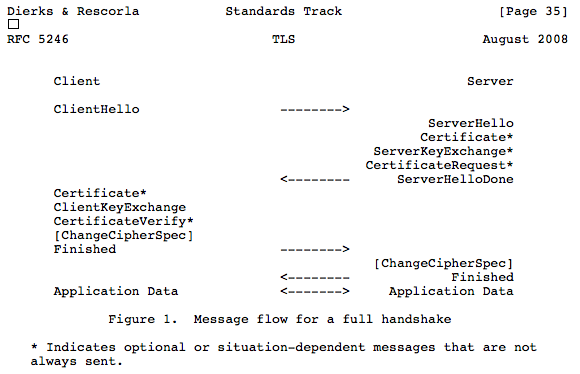
\includegraphics[width=\textwidth]{rfc5246.png}
\caption{The handshake illustrated in \href{https://tools.ietf.org/html/rfc5246#section-7.3}{RFC 5246} along with the extra-messages due to the ephemeral cipher-suite chosen}
\end{figure}

To attack the Server's ECDSA private key, we need it to sign a multitude of messages with that key. The easiest way to do this is to ask for an ephemeral connection. In Figure 5, you can see that when asking for an ephemeral cipher-suite in the ClientHello (DHE/ECDHE) you then get one extra message in the server's response: the \textbf{ServerKeyExchange} packet.

\begin{figure}[H]
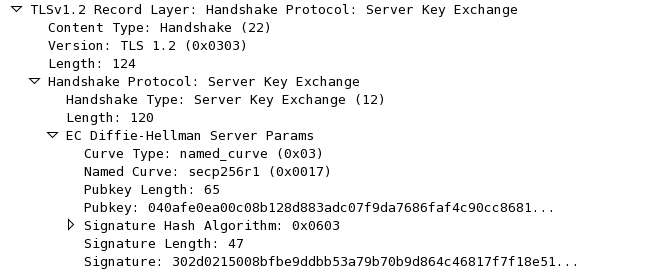
\includegraphics[width=\textwidth]{serverKeyExchange.png}
\caption{The serverKeyExchange packet parsed by WireShark}
\end{figure}

As you can see the server answers with a DSA/ECDSA signature, which is computed over a truncated hash of the ClientHello.random concatenated with ServerHello.random concatenated with the serverKeyExchange.params which are all available in clear during the handshake. And by the way, the fact that only the parameters and not the algorithm used in the Key Exchange are signed, is the cause of a long and old series of attack that had its more recent episode with the \textbf{Logjam attack}\cite{logjam}.

\begin{figure}[H]
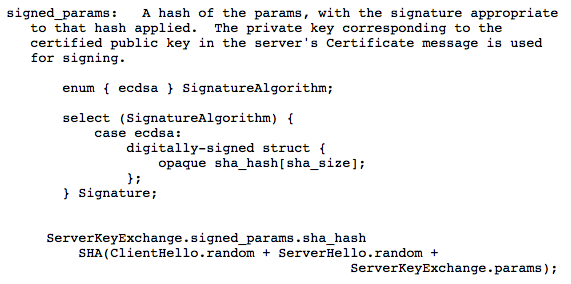
\includegraphics[width=\textwidth]{ecdsa_rfc4492.png}
\caption{The excerpt of \href{https://tools.ietf.org/html/rfc4492#section-5.4}{RFC 4492} talking about the signature part of an ephemeral handshake}
\end{figure}

The attack will consist of sending several ServerHello messages and collecting the signatures while timing the response time until enough small nonces are captured.

\subsection{Measuring a Timing Attack}

Since we are doing a remote attack, we cannot time the exact computation of the signature, what we time instead is the \textbf{round trip} time, defined by Crosby et al\cite{crosby} as such:
$$ \text{response\_time } = \text{ processing\_time } + \text{ propagation\_time } + \text{ jitter} $$

Here the \textit{processing\_time} is the difference between the target emitting its response and the target reading our helloClient. The nonce multiplication operation we want to time is in there and should be the only relevant computation in the overall timing of that part (i.e. all other server procedures' time are negligible compared to that multiplication operation). The \textit{propagation\_time} is the average time spent by the data in transit (i.e. between the attacker and the target). Finally, the \textit{jitter} is the uncontrollable noise/latency that can happen for many diverse reasons. The jitter is often the core problem of a remote timing attack.\\

To measure the timing of something, with extreme precision, we will rely on the \textbf{rdtscp} assembly instruction that returns the number of cycles the CPU has performed since boot. Contrary to rdtsc this operation does not need cpuid to be precise since rdtscp flushes the pipeline intrinsically. You only "need" to use cpuid and rdtsc if your processor does not support the more recent rdtscp, both requires a Pentium CPU.

\subsection{The Setup}

We modified \href{ftp://ftp.openssl.org/source/old/1.0.1/openssl-1.0.1j.tar.gz}{openssl-1.0.1j} to re-introduce the vulnerability by reverting the \href{https://git.openssl.org/?p=openssl.git;a=blobdiff;f=CHANGES;h=1633d27975c91f122c4e9266b2c3cf4e56e8ffbf;hp=22749650b701d91cc43af24a226369116c2a46f8;hb=992bdde62d2eea57bb85935a0c1a0ef0ca59b3da;hpb=bbcf3a9b300bc8109bb306a53f6f3445ba02e8e9}{patch from B.B.Brumley and N.Tuveri in OpenSSL 1.0.1j} as can be seen in figure \ref{fig:commented_patch}.

\begin{figure}[H]
\begin{minted}[breaklines,frame=single]{C}
/*
 * We do not want timing information to leak the length of k, so we
 * compute G*k using an equivalent scalar of fixed bit-length.
 */

/*
if (!BN_add(k, k, order))
    goto err;
if (BN_num_bits(k) <= BN_num_bits(order))
    if (!BN_add(k, k, order))
        goto err;
*/
\end{minted}
\caption{the patch commented in \textit{crypto/ecdsa/ecs\_ossl.c}}
\label{fig:commented_patch}
\end{figure}
Instead of creating a client packet that only allows for our ephemeral ECDSA handshake, we can use a server that only accepts that kind of ciphersuite. This is done with the OpenSSL command line tool and the following arguments:

\begin{minted}[breaklines,
 ]{bash}
$ openssl s_server -cert server.pem -key server.key -cipher "ECDHE-ECDSA-AES128-SHA256" -serverpref -quiet
\end{minted}

The \textit{-serverpref} argument allows us to force the server's ciphersuite on the client. Here we also use relevant server private and public keys that we generated with the following commands. Note that we chose the binary curve \textbf{sect163r2} but any binary curve should work (since they would use the same vulnerable code):

\begin{minted}[breaklines]{bash}
$ openssl ecparam -out server.key -name sect163r2 -genkey
$ openssl req -new -key server.key -x509 -nodes -days 365 -out server.pem
\end{minted}

And we obtain the certificate of figure 
\ref{fig:cert}.

\begin{figure}[H]
\begin{minted}[breaklines,frame=single]{bash}
$ openssl x509 -in server.pem -noout -text
Certificate:
Data:
    Version: 3 (0x2)
    Serial Number: 10869927066769118182 (0x96d9bd136d2d53e6)
Signature Algorithm: ecdsa-with-SHA256
    Issuer: C=US, ST=example@example.com, L=example@example.com, O=example@example.com, OU=example@example.com, CN=example@example.com/ emailAddress=example@example.com
    Validity
        Not Before: May  5 21:01:16 2015 GMT
        Not After : May  4 21:01:16 2016 GMT
    Subject: C=US, ST=example@example.com, L=example@example.com, O=example@example.com, OU=example@example.com, CN=example@example.com/ emailAddress=example@example.com
    Subject Public Key Info:
        Public Key Algorithm: id-ecPublicKey
            Public-Key: (163 bit)
            pub: 
            04:04:f3:e6:dd:ff:c4:ba:45:28:2f:3f:ab:e0:e8:                                    a2:20:b9:89:80:38:7a:05:d6:78:6b:3f:bd:8e:a7:                                    9c:b7:99:1c:d7:79:85:15:bb:cc:47:ce:54
            ASN1 OID: sect163r2
            NIST CURVE: B-163
    X509v3 extensions:
        X509v3 Subject Key Identifier: 
            35:B6:17:DC:06:42:19:C5:23:13:
            0E:35:26:AF:81:0C:E2:C4:91:B6
        X509v3 Authority Key Identifier: 
            keyid:35:B6:17:DC:06:42:19:C5:
            23:13:0E:35:26:AF:81:0C:E2:C4:91:B6

        X509v3 Basic Constraints: 
            CA:TRUE
Signature Algorithm: ecdsa-with-SHA256
     30:2e:02:15:03:f6:6a:a4:d4:e2:e5:80:30:bc:65:5a:da:32:
     5e:ab:b7:8b:fd:f6:88:02:15:01:fa:fa:23:59:f7:c1:23:d5:
     75:7c:a6:49:0b:d3:56:85:95:34:82:02
\end{minted}
\caption{The x509 certificate containing the binary curve as ECDHE/ECDSA parameters we generated with OpenSSL}
\label{fig:cert}
\end{figure}

\subsection{From the Server (the Target)}

We first modified OpenSSL to store the nonces it signed and how long it took to sign them. We then queried that server many times to make it use the ECDSA nonce multiplication operation. It took us 6 to 7 seconds to fetch 1,000 signatures and around a minute to fetch 10,000 signatures from the server.

\begin{figure}[H]
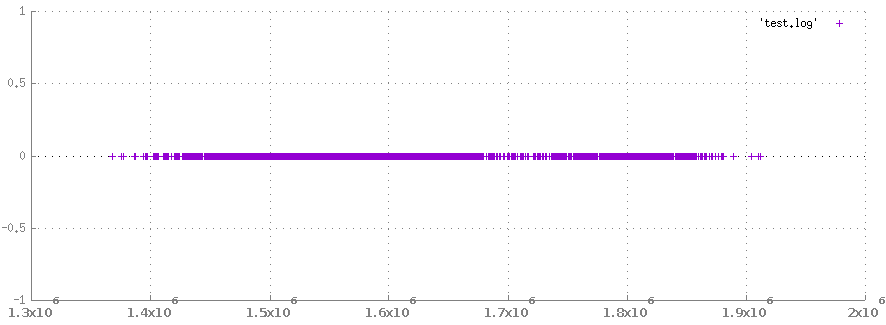
\includegraphics[width=\textwidth]{serverside_scrambled.png}
\caption{Every point is a signature, plotted according to the time it took the server to compute it in clock cycles (x axis)}
\end{figure}

After obtaining all the nonces and the timings, we plotted them and displayed the result in figure \ref{fig:serverside} to see that there was indeed a timing vulnerability in the ECDSA signature of OpenSSL for binary curves.

\begin{figure}[H]
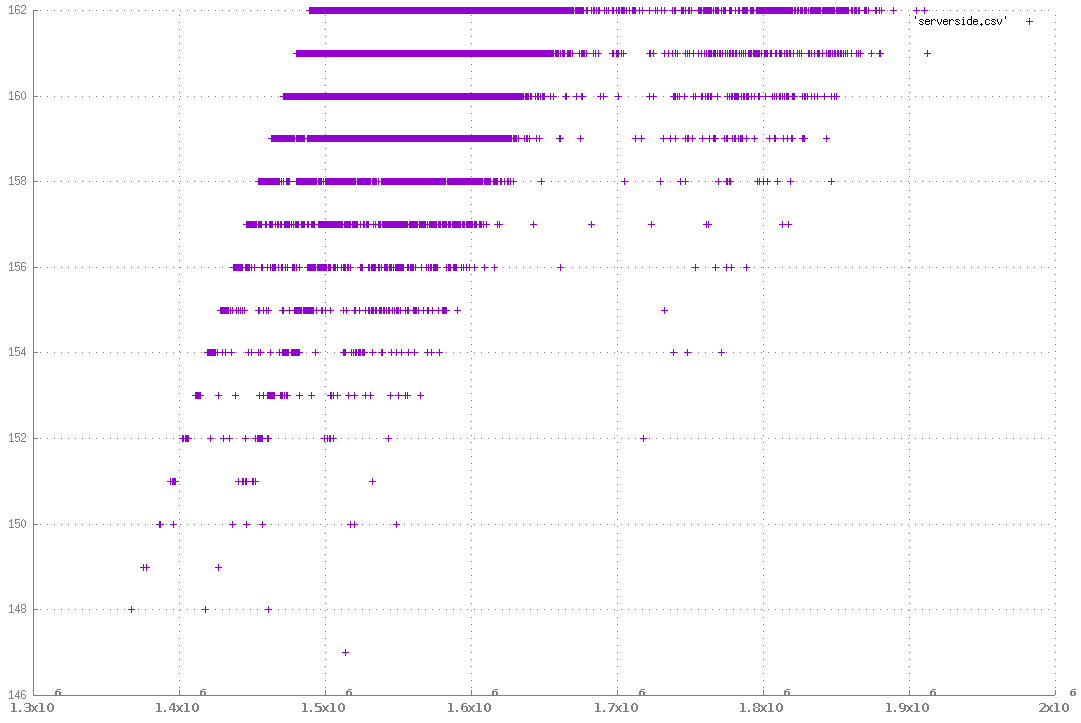
\includegraphics[width=\textwidth]{serverside.png}
\caption{The same graph where the signatures have been sorted by the binary length of the nonce (y axis)}
\label{fig:serverside}
\end{figure}

Finally we did some statistics on the amount of short nonces, the statistics were approximately the same for 1,000 and for 10,000 signatures:

\begin{figure}[H]
\begin{center} 
\begin{tabular}{@{} *2c @{}}
\toprule
 Length & Percentage \\ 
\midrule
$<157$&     0          \\
157&     1          \\
158&     3          \\
159&     6          \\
160&       13         \\
161&     24         \\
162&        50
\bottomrule
\end{tabular}
\end{center} 
\caption{Statistics on nonces generated for 1,000 signatures}
\end{figure}
These percentages are rounded and that shows that short nonces are pretty rare, here's a better table showing the amount of short nonces for 10,000 signatures requested:

\begin{figure}[H]
\begin{center} 
\begin{tabular}{@{} *2c @{}}
\toprule
length & amount \\ 
\midrule
146 &    1      \\
150&     1       \\
151 &    4       \\
152  &   8       \\
153   &  12      \\
154  &   12      \\
155 &    41      \\
156&     90      \\
157 &    141     \\
158 &    319     \\
159  &   624     \\
160   &  1259    \\
161    & 2503   \\ 
162     &4985    
\bottomrule
\end{tabular}
\end{center} 
\caption{Statistics on nonces generated for 10,000 signatures}
\end{figure}

We will discuss in the following sections how many nonces we need to perform the lattice attack.


\subsection{From a Remote Machine}

We tried getting the same kind of results from a different server located in the same local network. But as to simplify testing and avoid parsing the responses, we modified the OpenSSL server as to store the truncated hashes and the signatures server side.

The source code of the client is in Appendix A, it always sends the same \textit{HelloClient} packet (and the same \textit{client.Random}). The client counts the CPU cycles of the response time. If the attack is performed from multiple machines with different CPU frequencies then we would have to convert the CPU cycles into a time unit before gathering the data together.

Several ways of increasing the accuracy of these measurements were researched. The easiest thing is to configure the client machine that is in our control. Decreasing the jitter is often impossible since it happens out of our reach, getting close to the server seems to be the best way to do it, although our results are still inconclusive in a local network test environment as you will see later.

The program is run with the \textit{taskset} tool to avoid using multiple CPU, along with some kernel options like \textit{isolcpus} to avoid interruptions on the CPU we are using to make the measurements. The frequency scaling on that same CPU is disabled to avoid inconsistently counting CPU cycles. The program sends all but one byte, then sends the last byte and starts the \textit{rdtscp} counter. The counter is stopped as soon as the first byte is received. To do this we also need to disable \textit{Nagel's algorithm} on the socket we are using to disable network optimizations.

After collecting all the signatures we get rid of the 10 first samples and their imprecision due to the server cache warming up.

\begin{figure}[H]
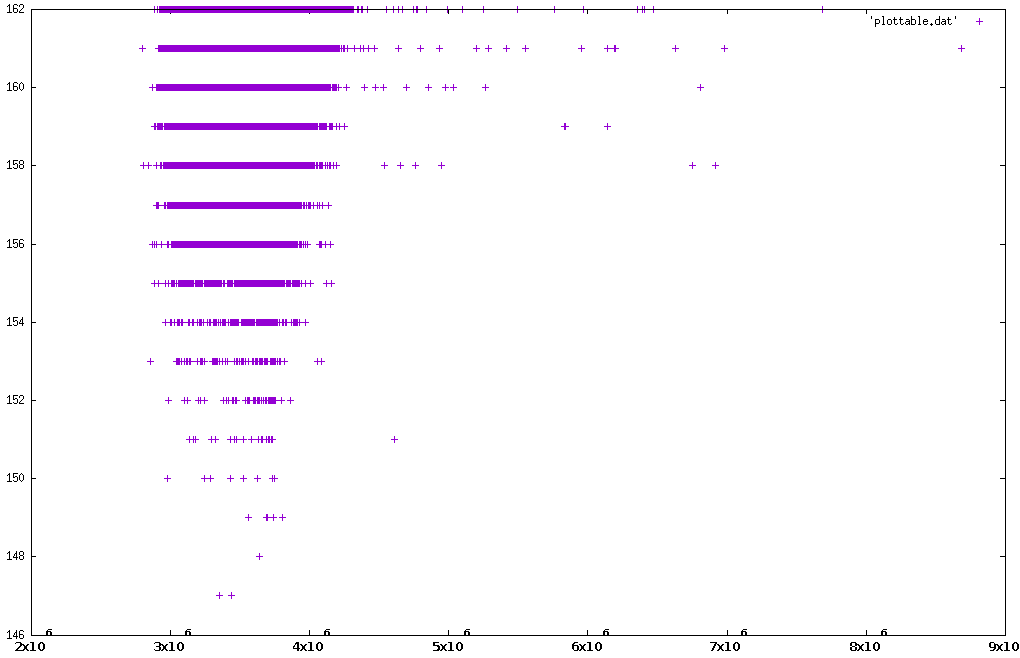
\includegraphics[width=\textwidth]{fail.png}
\caption{the y axis represents the bitsize of the nonces, the x axis the time the OpenSSL server took to respond. They are obviously not correlated}
\end{figure}

Retrieving 500 tuples (signatures and truncated digests) that took the smallest amount of time from 100,000 signatures, we can see that we do not have enough nonces of small sizes in our set (see next section on the lattice attack for numbers), plus the amount of false-positive is extremely high. We then try to get the smallest time upper-bound that would contain enough small nonces. We arrive at approximately 5,000: the fastest 5,000 signatures of our 100,000 signatures set should contain enough small nonces to do our lattice attack. And as we can see in figure 15 and in the following statistics, the amount of false positive is still extremely high.

\begin{table}[H]
\parbox{.45\linewidth}{
\centering
\begin{tabular}{@{} *3c @{}}
\toprule
length&amount&percentage\\
\midrule
150  &   1   &    0\\
152  &   1  &     0\\
153  &   1  &     0\\
154  &   3  &     0\\
155  &   10  &    2\\
156  &   11  &    2\\
157   &  18  &    3\\
158  &   27 &     5\\
159  &   42 &     8\\
160  &   89  &    17\\
161  &   113 &    22\\
162  &   184 &    36\\
\bottomrule
\end{tabular}
\caption{Stats on the nonces that computed the fastest 500 signatures}
}
\hfill
\parbox{.45\linewidth}{
\centering
\begin{tabular}{@{} *3c @{}}
\toprule
length&amount&percentage\\
\midrule
150  &   1     &  0\\
151   &  1  &     0\\
152  &   3 &      0\\
153   &  14  &    0\\
154  &   14 &     0\\
155  &   41 &     0\\
156   &  69  &    1\\
157  &   134    & 2\\
158   &  212&     4\\
159   &  388 &    7\\
160  &   721 &    14\\
161  &   1252   & 25\\
162    & 2150 &   43\\
\bottomrule
\end{tabular}
\caption{Stats on the nonces that computed the fastest 5,000 signatures}
}
\end{table}

To eliminate the false positives, the idea here is to select a random subset of let's say 42 tuples (if we are aiming for nonces smaller than 156 bits) and do a lattice attack, if we do not find anything build another random subset of the same size. Rinse and repeat. This leads to $1.36 \times 10^{104}$ different combinations, this is impossible and this is because our timing measurements are not correlated to the bitsize of the nonces. With better measurements this attack would indeed be devastating.

\subsection{The Lattice Attack}

Obviously our attack is not going to work from a remote machine because our timings are not correlated with the length of the nonces. We can try a theoretic attack by selecting the nonces by hand.

The code for the lattice attack can be found in Appendix B, it uses \textbf{Sage} and the embedding strategy talked about earlier.

In our experiments, we cannot solve for nonces greater than 157 bits (6 bits known). LLL also often provides worse results than \textbf{BKZ}. BKZ is another algorithm that approximate a solution for the SVP, it uses LLL but ends up with a smaller basis most of the time.

When only 6 bits are known, BKZ needs a minimum of 50 tuples (signatures and truncated hashes) to find the nonces, LLL needs 78. For nonces of 156 bits (7 bits are known), LLL starts needs a minimum of 42 tuples to find the values of the nonces whereas BKZ only needs 38. For nonces of bitsize 155, BKZ needs 30 tuples and LLL needs 31.

\begin{figure}[H]
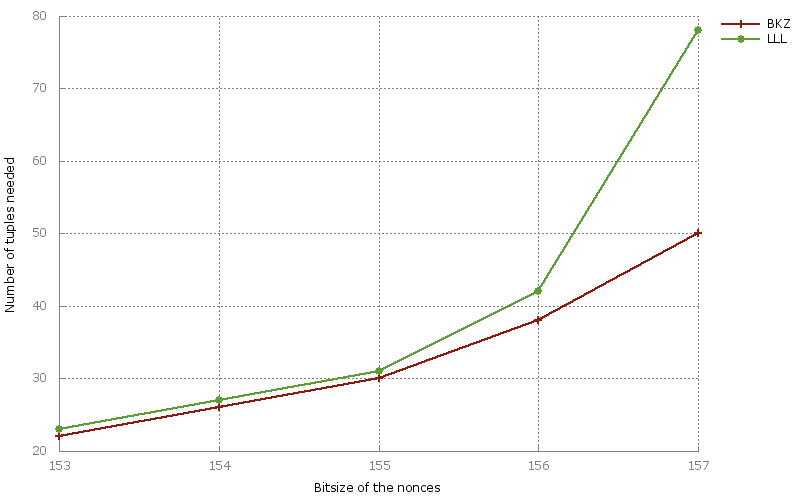
\includegraphics[width=\textwidth]{nice_web_plot.png}
\caption{The number of tuples needed by each algorithms (BKZ and LLL) according to the size of the nonces they can find}
\end{figure}

As seen in that kind of attacks in the literature, we use $q / 2^{l + 1}$ (with $q$ the modulo and $l$ the MSB (Most Significant Bits) known) for the trick in the embedding strategy. Using other values for the trick often provides worse results (more tuples are needed, or no solutions can be found), and if we do not use the extra dimension we cannot seem to find correct solutions.

\section{Countermeasures}

These kind of ``relaxed'' attacks on DSA and ECDSA are even more problematic on smart-cards, embedded devices and other cryptographic devices that can leak way more information through tons of other Side-Channel analysis. But to attack a remote target, timing attack is still one of the only reliable ways (along with the leak of information different error messages can give away). A relaxed remote attack model where the attacker shares the same machine as the victim can use such techniques as well. Some research have been done in Hypervisors where you could access information about neighbor VM's memory use\cite{flushreload}\cite{flushreloadecdsa}\cite{flushreloadopenssl}. The questions of ``Are there other kinds of side-channel attacks on remote targets?'' and ``Can we get more accurate timings on the network?'' are still open. As for the way of preventing timing attacks, a lot of countermeasures already exist.

\subsection{The OpenSSL Patch}

Let's first take a look at the fix proposed by B.B.Brumley and N.Tuveri following their finding.

\begin{figure}[H]
\begin{minted}[breaklines,frame=single]{C}
/* get random k */
do
    if (dgst != NULL) {
        if (!BN_generate_dsa_nonce
            (k, order, EC_KEY_get0_private_key(eckey), dgst, dlen,
             ctx)) {
            ECDSAerr(ECDSA_F_ECDSA_SIGN_SETUP,
                     ECDSA_R_RANDOM_NUMBER_GENERATION_FAILED);
            goto err;
        }
    } else {
        if (!BN_rand_range(k, order)) {
            ECDSAerr(ECDSA_F_ECDSA_SIGN_SETUP,
                     ECDSA_R_RANDOM_NUMBER_GENERATION_FAILED);
            goto err;
        }
    }
while (BN_is_zero(k));

/*
 * We do not want timing information to leak the length of k, so we
 * compute G*k using an equivalent scalar of fixed bit-length.
 */

if (!BN_add(k, k, order))
    goto err;
if (BN_num_bits(k) <= BN_num_bits(order))
    if (!BN_add(k, k, order))
        goto err;

/* compute r the x-coordinate of generator * k */
if (!EC_POINT_mul(group, tmp_point, k, NULL, NULL, ctx)) {
\end{minted}
\caption{the patch of B.B.Brumley and N.Tuveri in \textit{crypto/ecdsa/ecs\_ossl.c}}
\end{figure}

The attack we presented works because some of the nonces are short enough. A solution could be to \textbf{make them all long enough} so that the underlying lattice attack could not happen. This is what B.B.Brumley and N.Tuveri proposed, and is facilitated by the properties of the scalar multiplication in Elliptic Curve Cryptography:

$$ [k]P = [k + r]P \text{ if } r \text{ is a multiple of the group order} $$

As we will see later, this property is often used as \textbf{scalar blinding} against Side-Channel Attacks. But rather than using a random multiple of the group order which would make extremly large nonces, we can just add the group order to the nonce once. If it's not long enough, the second test will add the group order once again. This will be enough to avoid short nonces all of the time.

\subsection{Blinding}

In 1996, Kocher\cite{Kocher} introduced a timing attack on Diffie-Hellman, RSA and DSA, revant countermeasure: \textbf{blinding}. He explained two ways of using it, either as a base blinding, or as an exponent blinding (although it was shown that under certain conditions exponent blinding alone was not sufficient\cite{schindler}). Both techniques allow the operation to be computed on something unrelated to a malicious user's controlled input.\\

Below is the \textbf{base blinding} technique applied during a RSA decryption phase with $m = c^d \mod{N}$ where $m$ is the message, $c$ is the ciphertext, $d$ is the private exponent and $N$ the modulus:

\begin{enumerate}
\item{$r  \xleftarrow[]{\$} \mathbb{Z}_N^{\ast}$}
\item{$m' = (c \cdot r^e)^d \pmod{N}$}
\item{$m = m' \cdot r^{-1} \pmod{N}$}
\end{enumerate}

To harden base blinding, \textbf{exponent blinding} can be added. Instead of randomizing the ciphertext, the idea is to randomize the private exponent by adding it to a multiple of $\varphi(N)$:

\begin{enumerate}
    \item{$k \xleftarrow[]{\$} \mathbb{Z}$}
    \item{$d' = c^{d + k \cdot \varphi(N)} \pmod{N}$}
    \item{$m = c^{d'} \pmod{N}$}
\end{enumerate}

In cryptosystems based on Elliptic Curve Cryptography, other forms of blinding can be used, we will first re-introduce scalar blinding. Here in $Q = [d]P$ we have $P=(x,y)$:

\textbf{Scalar blinding} is the exponent blinding of RSA, in $Q = [d]P$ you hide the private key by adding it to a multiple of the group order.

\begin{enumerate}
\item{$k \xleftarrow[]{\$} \mathbb{Z}$}
\item{$k d' = d + k \cdot \#E(\mathbb{F}_q)$ the order of the curve}
\item{$Q = [d']P$}
\end{enumerate}

\textbf{Coordinate blinding} is another form of blinding aimed to express calculations in a different projective coordinate every time:

\begin{enumerate}
\item{$k \xleftarrow[]{\$} \mathbb{Z}$}
\item{Compute $P = (kx, ky, k)$ expressed by projective coordinates.}
\item{Compute $[d]P$ using the scalar multiplication algorithm with projective coordinates on the Montgomery-form elliptic curve.}
\item{Output $[d]P$}
\end{enumerate}

\textbf{Point blinding} is the base blinding of ECC, in $Q = [d]P$ you hide the base point $P$ by adding it to a random point:

\begin{enumerate}
\item{$S \xleftarrow[]{\$} E(\mathbb{F}_q)$}
\item{Compute $S' = [d]S$}
\item{$Q' = [d](P + S)$}
\item{$Q = Q' - S'$}
\end{enumerate}

\subsection{Constant-Time}

Another popular way of preventing against timing attacks is to use Constant-Time algorithms like we have seen with OpenSSL's ECDSA implementation for binary curves. It is also often used for comparing MACs or Signatures together without leaking information on the bytes of the correct string, by failing as soon as a byte is not the same.\\

Constant-Time exponentiation in modular arithmetic based cryptosystems like DH are done with \textbf{Square-and-Multiply-Always}, which is a modified Square-and-Multiply algorithm that does both operations every time. Here we are decrypting a ciphertext $c$ with the operation $c^d \pmod{N}$ where $d$ is the private key, $|d|$ its binary length and $d_i$ the number at the i-th position of its binary representation.

\DontPrintSemicolon
\begin{algorithm}[H]
    $s = 1$\;
    \For{$i$ from $|d|-1$ down to $0$}{
        $s = s * s \mod{N}$ \;
        \lIf{$d_i = 1$}{
            $s = s \cdot c \pmod{N}$ 
        }
        \lElse{
            $t = s \cdot c \pmod{N}$
        }
    }
    return $s$\;
\end{algorithm}

Constant-Time in ECC, usually applied on multiplication operations, are done with the \textbf{Double-and-Add-Always} or the \textbf{Montgomery Ladder} algorithm like in the OpenSSL's ECDSA implementation for binary curves. Both are exactly the same idea as the Square-and-Multiply-Always were dummy operations are made.\\
Here is the Montgomery Ladder algorithm:

\begin{algorithm}[H]
    $R_0 = 0$\;
    $R_1 = P$\;
    \For{$i$ from $|d|-1$ down to $0$}{
        \uIf{$d_i = 0$}{
	        $R_1 = R_0 + R_1$\;
	        $R_0 = 2R_0$\;
        }
        \Else{
	        $R_0 = R_0 + R_1$\;
	        $R_1 = 2R_1$\;
        }
    }
    return $R0$\;
\end{algorithm}

\subsection{Others}

We will briefly talk about the other alternatives to the previous two popular ones.\\

The \textbf{Unified Formula} technique intends to make point addition and point doubling use the same sequence of field operations. It was first invented by Brier and Joye in 2002\cite{unified} and is aiming to cancel the problems brought by the difference of operations occurring in $P + Q$ when $P = Q$.\\

Another relatively new technique is the \textbf{Padding-Time} technique, which was introduced in 2015 by Boneh, Braun and Jana. The idea is to always take the same amount of time by waiting before doing anything else if an operation did not take as much time as its precedents.\\

A totally different take on this problem is to get rid of the randomness of the nonces by \textbf{deterministically deriving the nonces from the message and some secret data}. There are two main propositions in this field: the D.J.Bernstein's one with EdDSA\cite{eddsa}, which completely changes ECDSA (uses different curves), and Thomas Pornin's\cite{pornin} one which generate the nonces with HMAC in the ECDSA.

\section{Conclusion}

We have seen in our own experiments that Remote timing attacks are \textbf{far from being practical}, even in the same local network. It already takes advanced measures to attain high precision of timings on the attacker machine, and the fact that we cannot control the jitter, the propagation time and the overall server's responsiveness make things extremely difficult for us.\\

It's important to notice that the lattice attack should still have \textbf{room for improvement} and more resources would make the timing attack more efficient as well. The detailed and respected description of the TLS protocol would make such a potentially efficient attack particularly easy to perform against any TLS framework/library having such vulnerability.\\ \href{http://blog.cryptographyengineering.com/2012/03/surviving-bad-rng.html}{Some cryptographers} have already advised not to use ECDSA to cryptographically sign objects. The topic is currently a hot one in the \href{http://www.ietf.org/mail-archive/web/cfrg/current/maillist.html}{CFRG mailing list} as what new Signature scheme should become the standard in the years to come.

\newpage

\begin{thebibliography}{1}

\bibitem{ps3} PS3 Nonce Re-use {\em http://www.bbc.com/news/technology-12116051}

\bibitem{Kocher} Paul C. Kocher {\em Timing Attacks on Implementations of Diffie-Hellman, RSA, DSS, and Other Systems}

\bibitem{brumley-tuveri} B.B.Brumley and N.Tuveri {\em Remote Timing Attacks are Still Practical}

\bibitem{boneh-venkatesan} D. Boneh and R. Venkatesan {\em Hardness of computing the most significant bits of secret keys in Diffie-Hellman and related schemes}

\bibitem{HG-smart} N.A.Howgrave-Graham and N.P.Smart {\em Lattice Attacks on DSA}

\bibitem{dualec} Daniel J. Bernstein, Tanja Lange, and Ruben NiederhagenDual {\em EC: A Standardized Back Door}

\bibitem{babai} László Babai {\em On Lovász' lattice reduction and the nearest lattice point problem}

\bibitem{crosby} Scott A. Crosby, Dan S. Wallach, and Rudolf H. Riedi {\em Opportunities and Limits of Remote Timing Attacks}

\bibitem{chrispeikert} Chris Peikert {\em Lattices in Cryptography, Georgia Tech, Fall 2013: Lecture 2, 3}

\bibitem{logjam} David Adrian, Karthikeyan Bhargavan, J. Alex Halderman, Nadia Heninger, Benjamin VanderSloot, Eric Wustrow, Zakir Durumeric, Pierrick Gaudry, Matthew Green, Drew Springall, Emmanuel Thome,† Luke Valenta, Santiago Zanella-Bégulin, Paul Zimmermann {\em Imperfect Forward Secrecy: How Diffie-Hellman Fails in Practice}

\bibitem{coppersmith} Don Coppersmith {\em Finding Small Solutions to Small Degree Polynomials}

\bibitem{lll} Lenstra, A. K.; Lenstra, H. W., Jr.; Lovász, L. (1982). {\em "Factoring polynomials with rational coefficients"}

\bibitem{flushreload} Yarom, Falkner {\em FLUSH+RELOAD: a High Resolution, Low Noise, L3 Cache Side-Channel Attack}

\bibitem{ecdsa} Johnson, Menezes, Vanstone {/em The Elliptic Curve Digital Signature Algorithm (ECDSA)}

\bibitem{flushreloadecdsa} Benger, van de Pol, Smart, Yarom {\em “Ooh Aah... Just a Little Bit” : A small amount of side channel can go a long way}

\bibitem{flushreloadopenssl} Yarom, Benger {\em Recovering OpenSSL ECDSA Nonces Using the FLUSH+RELOAD Cache Side-channel Attack}

\bibitem{schnorr} Schnorr (1989) {\em Efficient Identification and Signatures for Smart Cards}

\bibitem{schindler} Werner Schindler {\em Exclusive Exponent Blinding May Not Suffice to Prevent Timing Attacks on RSA}

\bibitem{pornin} Thomas Pornin {\em Deterministic Usage of the Digital Signature Algorithm (DSA) and Elliptic Curve Digital Signature Algorithm (ECDSA)}

\bibitem{eddsa} D.J.Bernstein {\em High-speed high-security signatures}

\bibitem{unified} Brier, Joye {\em Weierstraß elliptic curves and side-channel attacks}

\end{thebibliography}

\newpage

\appendix 

\section{Timing Attack in C}

\inputminted[breaklines]{c}{attack.c}

\newpage

\section{Lattice Attack in Sage}

\inputminted[breaklines]{sage}{lattice.sage}

\end{document}